% !TeX program = lualatex
\documentclass[a0paper,landscape]{baposter}

\usepackage[EU1]{fontenc}
\usepackage{fontspec}
\defaultfontfeatures{Ligatures=TeX}
\setromanfont{TeX Gyre Schola}
\setsansfont{TeX Gyre Adventor}
\setmonofont{TeX Gyre Cursor}
\usepackage{microtype}

\usepackage{setspace}

\usepackage{fancyvrb}

% TODO change this
\usepackage{lyluatex}

\definecolor{lilyLightHeader1}{RGB}{212,242,201}
\definecolor{lilyLightHeader2}{RGB}{140,210,118}
\definecolor{lilyDarkHeader}{RGB}{91,127,100}


\begin{document}
\begin{poster}{%
	columns=5,
	background=none,
  % Show grid to help with alignment
	grid=false,
% Column spacing
	colspacing=1em,
% Color style
	bgColorOne=white,
	bgColorTwo=lilyLightHeader1,
	borderColor=lilyDarkHeader,
	headerColorOne=white,
	headerColorTwo=lilyLightHeader1,
	headerFontColor=lilyDarkHeader,
	boxColorOne=lilyLightHeader1,
	boxColorTwo=lilyLightHeader2,
% Format of textbox
	textborder=faded,
% Format of text header
	eyecatcher=true,
	headerborder=closed,
	headerheight=0.1\textheight,
    % textfont=\sc, % An example of changing the text font
	headershape=rounded,
	headershade=shadetb,
    % headerfont=\Large\bf\textsc, %Sans Serif
    % textfont={\setlength{\parindent}{1.5em}},
	boxshade=plain,
%   background=shade-tb,
	background=plain,
	linewidth=2pt
	}
% eyecatcher
  {
  	
\includegraphics[width=0.11\linewidth]{double-lily-modified3.png}
  }
% title
  {GNU LilyPond}
% author
  {}
% university
  {
\includegraphics[width=.11\textwidth]{double-lily-modified3.png}}
%%%%%%%%%%%%%%%%%%%%%%%%%%%%%%%%%%%%%%%%%%%%%%%%%%%%%%%%%%%%%%%%%%%%%%%%%%%%%%%
%%% Content

  \headerbox{Text Input}{name=text,column=0,span=1,boxpadding=12pt}{
LilyPond is a compiled system: it is run on a text file describing the music. The resulting output is viewed on-screen or printed. In some ways, LilyPond is more similar to a programming language than graphical score editing software.

You do not write music by dragging notes from a graphical toolbar and placing them on a dynamically refreshing score; you write music by typing text. This text is interpreted (or “compiled”) by LilyPond, which produces beautifully engraved sheet music.

People accustomed to graphical user interfaces might need to learn a new way of working, but the results are definitely worth it!
  }

\headerbox{Note Entry}{name=text,column=0,span=1,boxpadding=12pt,below=text}{
	Note entry is as easy as typing the note name and the duration.

	\VerbatimInput{lily/note-entry.ly}

	\lilypondfile{lily/note-entry.ly}

	Just type the note name \texttt{c, d, e, f, g, a, b}, append \texttt{is} for sharp and \texttt{es} for flat tones and add the duration with 4 for fourth, 8 for eigth and so on. With one or more dots you
	create dotted notes. Pitch is specified using a variant of the Helmholtz pitch notation.

}

\headerbox{Note Entry}{name=figures,column=1,span=1,boxpadding=12pt}{
	It is easy to add a figured bass.\vspace{1em}

	\texttt{<7\textbackslash+ 4 2>8 <8> <7!>}\vspace{1em}

    \lilypondfile{lily/figured-bass.ly}

}

  \headerbox{Classical Music}{name=classical,column=1,span=1,below=figures}{
  	Excerpt from the Markus Passion by Johann Sebastian Bach (BWV 247)

	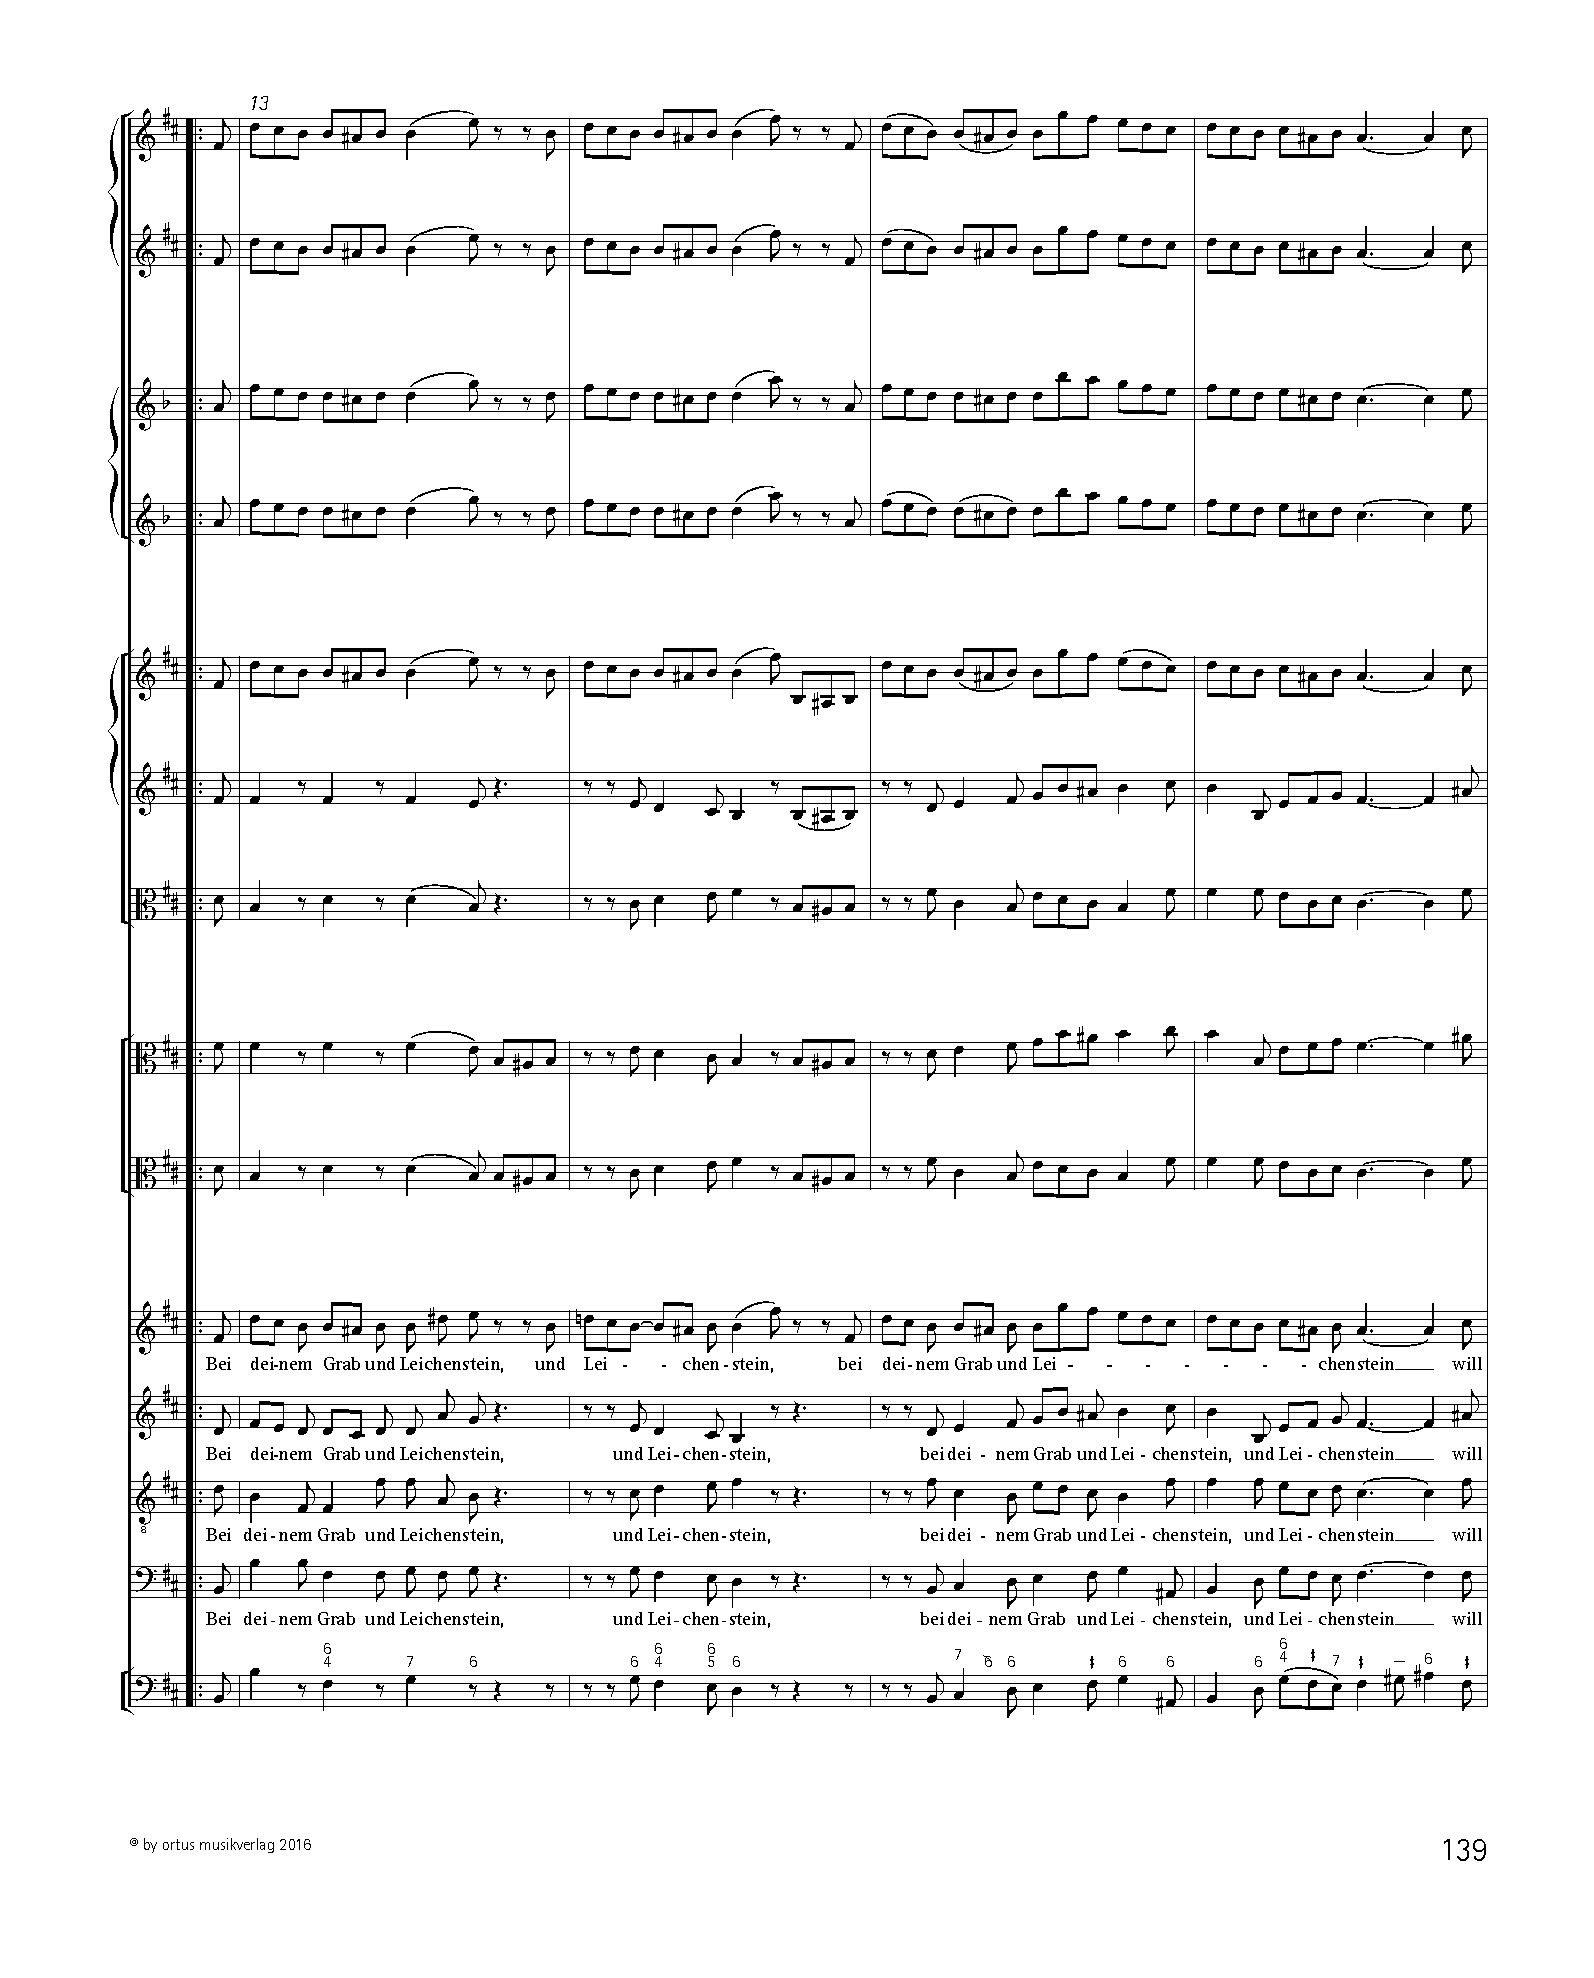
\includegraphics[width=\textwidth]{bwv247-partitur1.pdf}

	{\scriptsize © 2016 Ortus Musik Verlag, Berlin $\bullet$
	\emph{The excerpt is reproduced with the kind permission of the publisher.}}
  }

  \headerbox{Contemporary Music}{name=classical,column=3,span=1}{
	Excerpt from “All Things Rush On” by Kieren MacMillan

	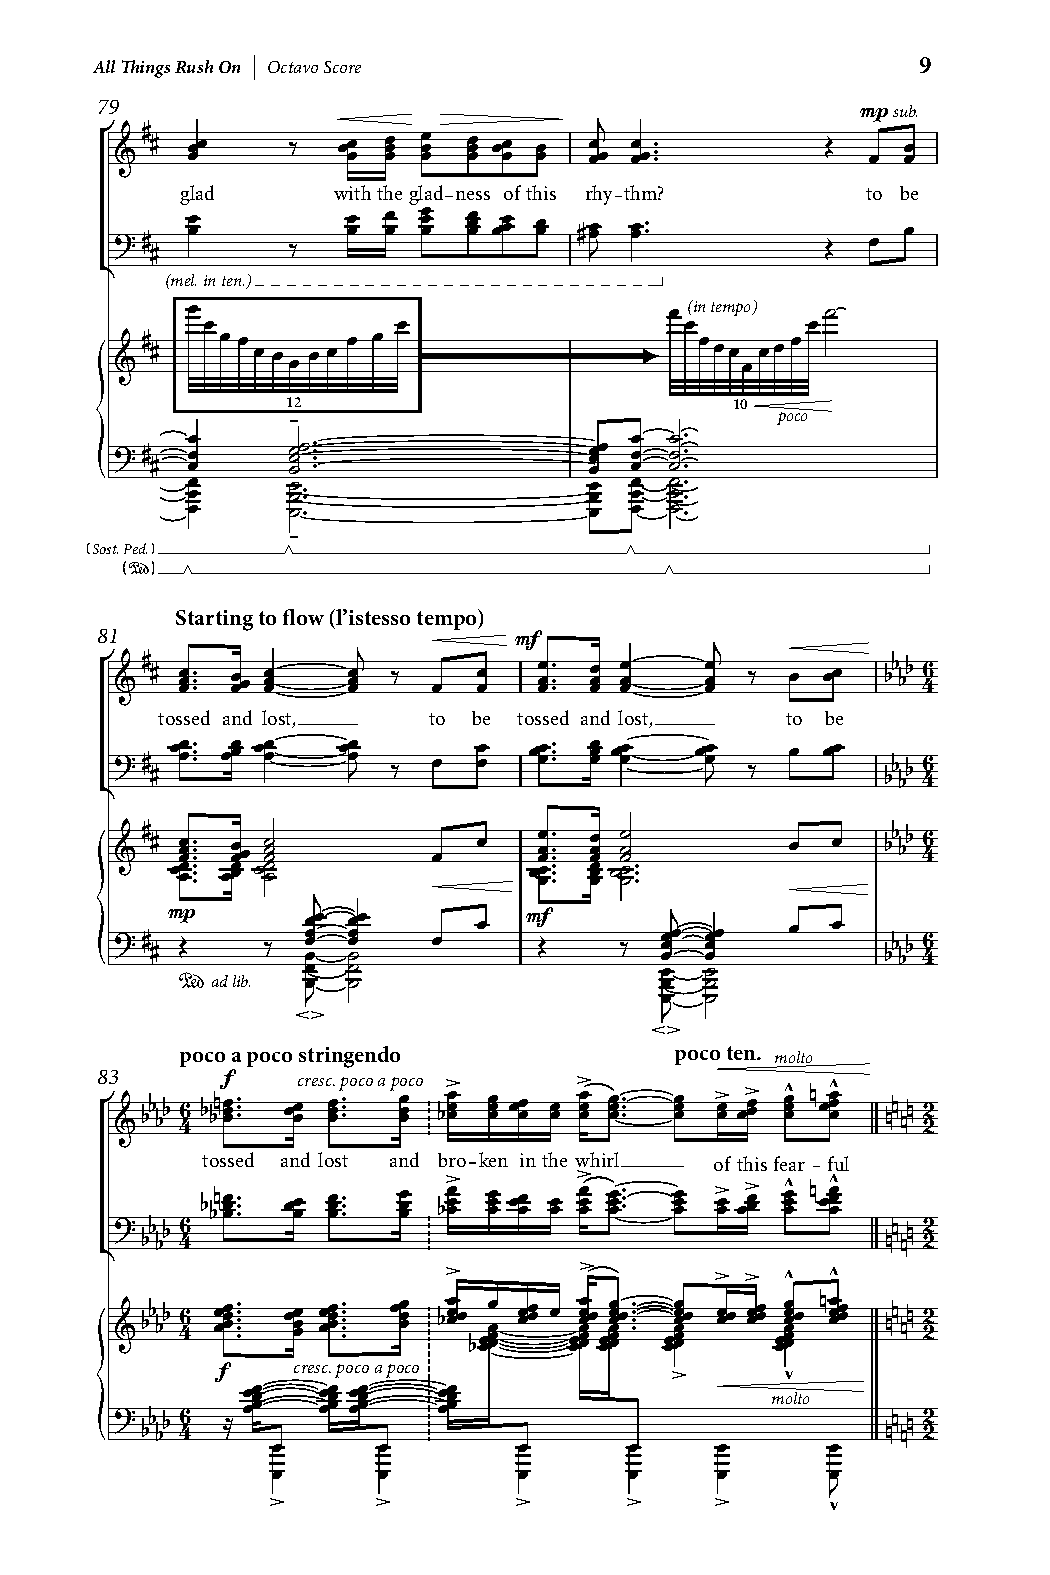
\includegraphics[width=\textwidth]{AllThingsRushOn_pg13.pdf}

	{\scriptsize © 2019 Kieren MacMillan $\bullet$
		\emph{The excerpt is reproduced with the kind permission of the publisher.}}
}

  \headerbox{Contemporary Music}{name=keller,column=4,span=1}{
	Excerpt from Hermann Keller's composition for speaking cellist\\
	»Ihr sollt die Wahrheit erben«

    %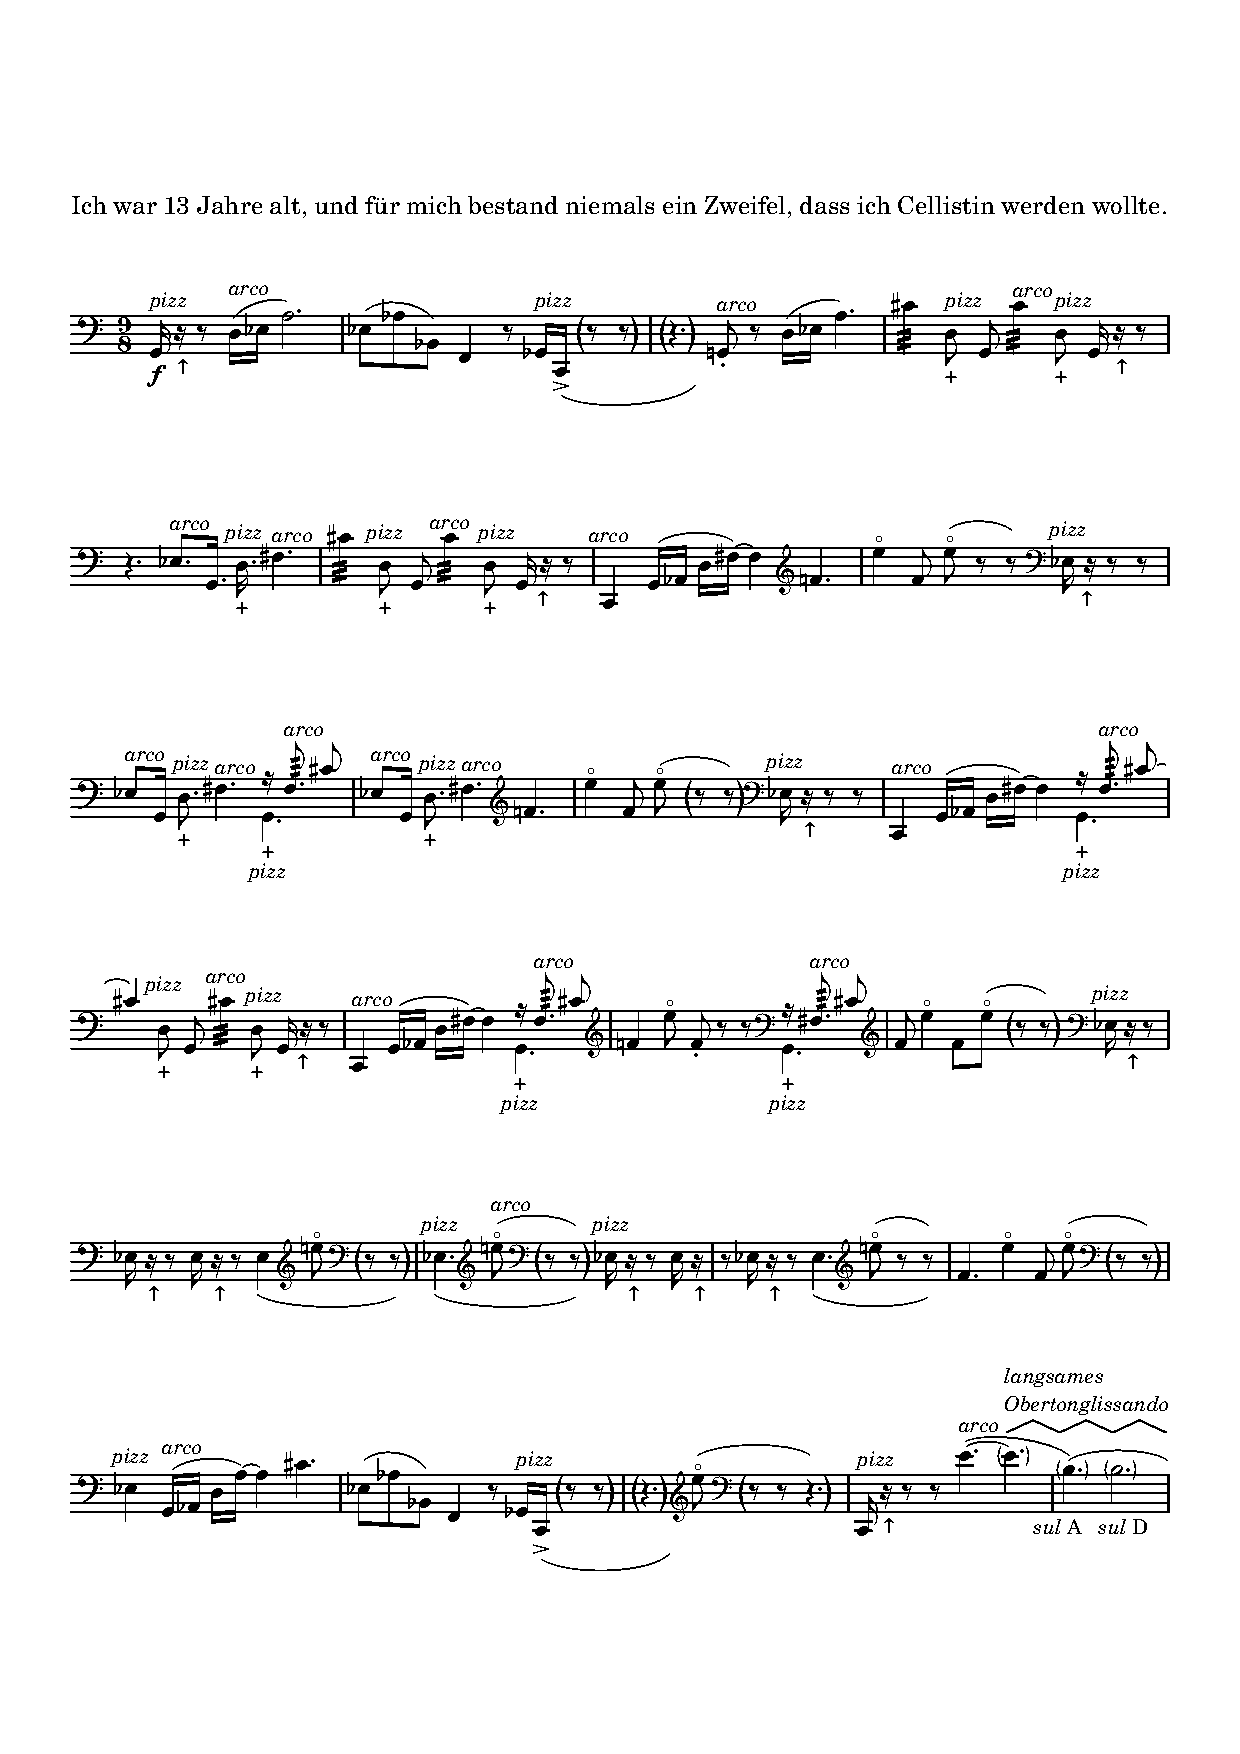
\includegraphics[width=.5\textwidth]{keller-wahrheit1}
    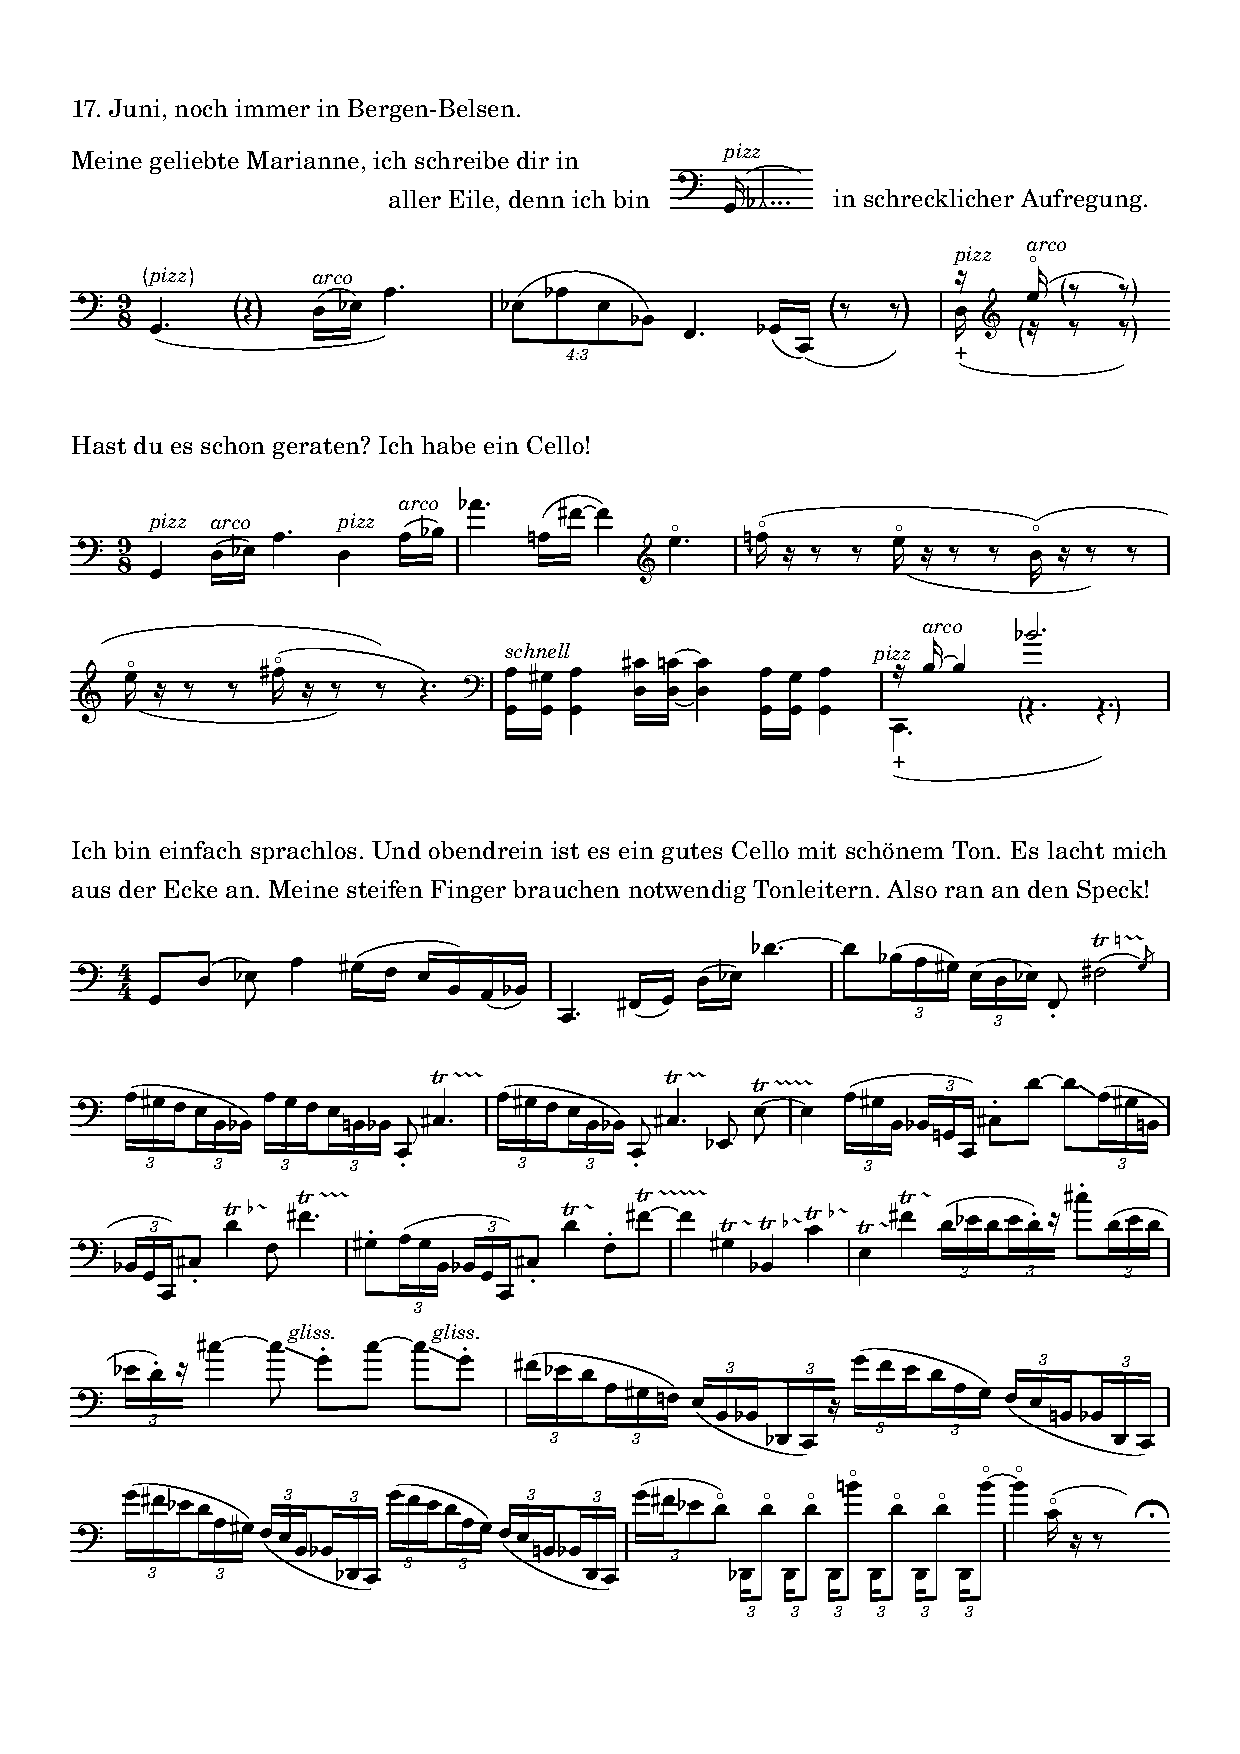
\includegraphics[width=\textwidth]{keller-wahrheit2}

	{\scriptsize © 2019 Edition Juliane Klein, Berlin $\bullet$
	\emph{The excerpt is reproduced with the kind permission of the publisher.}}
    }
  \headerbox{}{column=0,span=5,row=.885}{
  	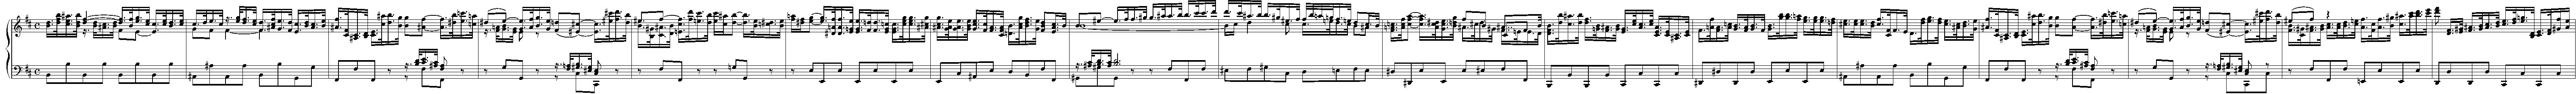
\includegraphics[width=\textwidth]{salzburg-poster.pdf}
  }

\end{poster}
\end{document}
